% Created by tikzDevice version 0.12
% !TEX encoding = UTF-8 Unicode
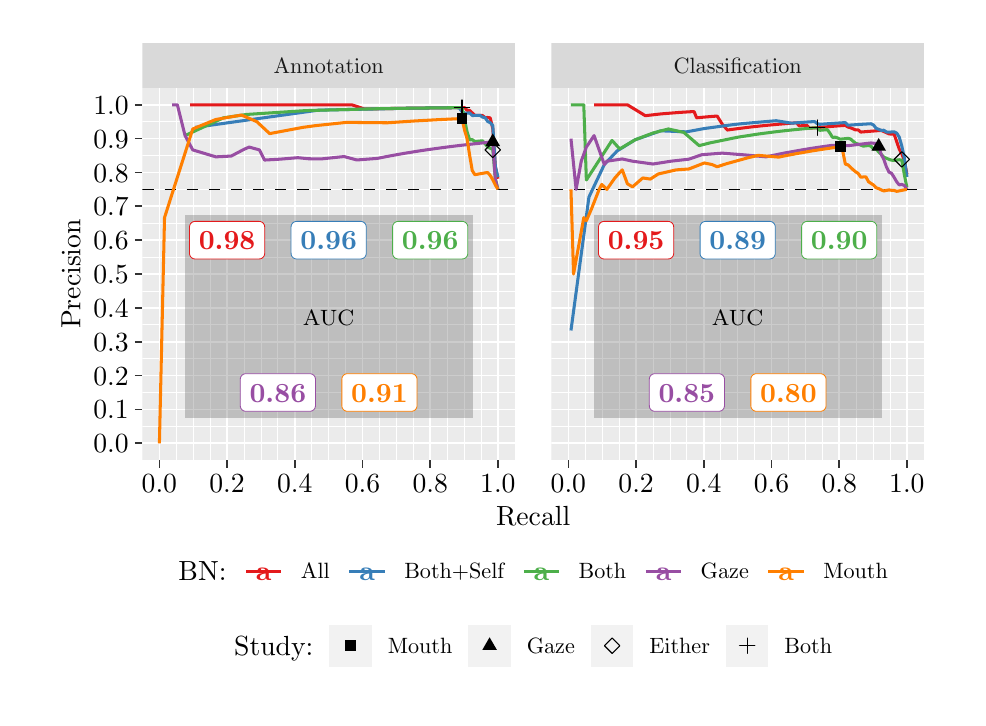
\begin{tikzpicture}[x=1pt,y=1pt]
\definecolor{fillColor}{RGB}{255,255,255}
\path[use as bounding box,fill=fillColor,fill opacity=0.00] (0,0) rectangle (336.00,242.28);
\begin{scope}
\path[clip] (  6.68,  0.00) rectangle (329.32,242.28);
\definecolor{drawColor}{RGB}{255,255,255}
\definecolor{fillColor}{RGB}{255,255,255}

\path[draw=drawColor,line width= 0.6pt,line join=round,line cap=round,fill=fillColor] (  6.68,  0.00) rectangle (329.32,242.28);
\end{scope}
\begin{scope}
\path[clip] ( 41.48, 85.99) rectangle (176.03,220.53);
\definecolor{fillColor}{gray}{0.92}

\path[fill=fillColor] ( 41.48, 85.99) rectangle (176.03,220.53);
\definecolor{drawColor}{RGB}{255,255,255}

\path[draw=drawColor,line width= 0.3pt,line join=round] ( 41.48, 98.22) --
	(176.03, 98.22);

\path[draw=drawColor,line width= 0.3pt,line join=round] ( 41.48,110.45) --
	(176.03,110.45);

\path[draw=drawColor,line width= 0.3pt,line join=round] ( 41.48,122.68) --
	(176.03,122.68);

\path[draw=drawColor,line width= 0.3pt,line join=round] ( 41.48,134.91) --
	(176.03,134.91);

\path[draw=drawColor,line width= 0.3pt,line join=round] ( 41.48,147.14) --
	(176.03,147.14);

\path[draw=drawColor,line width= 0.3pt,line join=round] ( 41.48,159.37) --
	(176.03,159.37);

\path[draw=drawColor,line width= 0.3pt,line join=round] ( 41.48,171.60) --
	(176.03,171.60);

\path[draw=drawColor,line width= 0.3pt,line join=round] ( 41.48,183.84) --
	(176.03,183.84);

\path[draw=drawColor,line width= 0.3pt,line join=round] ( 41.48,196.07) --
	(176.03,196.07);

\path[draw=drawColor,line width= 0.3pt,line join=round] ( 41.48,208.30) --
	(176.03,208.30);

\path[draw=drawColor,line width= 0.3pt,line join=round] ( 53.72, 85.99) --
	( 53.72,220.53);

\path[draw=drawColor,line width= 0.3pt,line join=round] ( 59.83, 85.99) --
	( 59.83,220.53);

\path[draw=drawColor,line width= 0.3pt,line join=round] ( 65.95, 85.99) --
	( 65.95,220.53);

\path[draw=drawColor,line width= 0.3pt,line join=round] ( 78.18, 85.99) --
	( 78.18,220.53);

\path[draw=drawColor,line width= 0.3pt,line join=round] ( 84.29, 85.99) --
	( 84.29,220.53);

\path[draw=drawColor,line width= 0.3pt,line join=round] ( 90.41, 85.99) --
	( 90.41,220.53);

\path[draw=drawColor,line width= 0.3pt,line join=round] (102.64, 85.99) --
	(102.64,220.53);

\path[draw=drawColor,line width= 0.3pt,line join=round] (108.76, 85.99) --
	(108.76,220.53);

\path[draw=drawColor,line width= 0.3pt,line join=round] (114.87, 85.99) --
	(114.87,220.53);

\path[draw=drawColor,line width= 0.3pt,line join=round] (127.10, 85.99) --
	(127.10,220.53);

\path[draw=drawColor,line width= 0.3pt,line join=round] (133.22, 85.99) --
	(133.22,220.53);

\path[draw=drawColor,line width= 0.3pt,line join=round] (139.33, 85.99) --
	(139.33,220.53);

\path[draw=drawColor,line width= 0.3pt,line join=round] (151.57, 85.99) --
	(151.57,220.53);

\path[draw=drawColor,line width= 0.3pt,line join=round] (157.68, 85.99) --
	(157.68,220.53);

\path[draw=drawColor,line width= 0.3pt,line join=round] (163.80, 85.99) --
	(163.80,220.53);

\path[draw=drawColor,line width= 0.6pt,line join=round] ( 41.48, 92.10) --
	(176.03, 92.10);

\path[draw=drawColor,line width= 0.6pt,line join=round] ( 41.48,104.33) --
	(176.03,104.33);

\path[draw=drawColor,line width= 0.6pt,line join=round] ( 41.48,116.56) --
	(176.03,116.56);

\path[draw=drawColor,line width= 0.6pt,line join=round] ( 41.48,128.80) --
	(176.03,128.80);

\path[draw=drawColor,line width= 0.6pt,line join=round] ( 41.48,141.03) --
	(176.03,141.03);

\path[draw=drawColor,line width= 0.6pt,line join=round] ( 41.48,153.26) --
	(176.03,153.26);

\path[draw=drawColor,line width= 0.6pt,line join=round] ( 41.48,165.49) --
	(176.03,165.49);

\path[draw=drawColor,line width= 0.6pt,line join=round] ( 41.48,177.72) --
	(176.03,177.72);

\path[draw=drawColor,line width= 0.6pt,line join=round] ( 41.48,189.95) --
	(176.03,189.95);

\path[draw=drawColor,line width= 0.6pt,line join=round] ( 41.48,202.18) --
	(176.03,202.18);

\path[draw=drawColor,line width= 0.6pt,line join=round] ( 41.48,214.41) --
	(176.03,214.41);

\path[draw=drawColor,line width= 0.6pt,line join=round] ( 47.60, 85.99) --
	( 47.60,220.53);

\path[draw=drawColor,line width= 0.6pt,line join=round] ( 72.06, 85.99) --
	( 72.06,220.53);

\path[draw=drawColor,line width= 0.6pt,line join=round] ( 96.52, 85.99) --
	( 96.52,220.53);

\path[draw=drawColor,line width= 0.6pt,line join=round] (120.99, 85.99) --
	(120.99,220.53);

\path[draw=drawColor,line width= 0.6pt,line join=round] (145.45, 85.99) --
	(145.45,220.53);

\path[draw=drawColor,line width= 0.6pt,line join=round] (169.91, 85.99) --
	(169.91,220.53);
\definecolor{drawColor}{RGB}{0,0,0}

\path[draw=drawColor,line width= 0.6pt,dash pattern=on 4pt off 4pt ,line join=round] ( 41.48,183.84) -- (176.03,183.84);
\definecolor{fillColor}{RGB}{89,89,89}

\path[fill=fillColor,fill opacity=0.30] ( 56.77,101.28) rectangle (160.74,174.66);

\node[text=drawColor,anchor=base,inner sep=0pt, outer sep=0pt, scale=  1.00] at (108.76,134.51) {\footnotesize{AUC}};
\definecolor{drawColor}{RGB}{255,127,0}
\definecolor{fillColor}{RGB}{255,255,255}

\path[draw=drawColor,line width= 0.3pt,line join=round,line cap=round,fill=fillColor] (115.52,103.67) --
	(138.69,103.67) --
	(138.61,103.67) --
	(138.93,103.69) --
	(139.24,103.75) --
	(139.54,103.86) --
	(139.82,104.02) --
	(140.07,104.23) --
	(140.28,104.47) --
	(140.45,104.74) --
	(140.57,105.03) --
	(140.65,105.34) --
	(140.68,105.66) --
	(140.68,105.66) --
	(140.68,115.24) --
	(140.68,115.24) --
	(140.65,115.56) --
	(140.57,115.87) --
	(140.45,116.16) --
	(140.28,116.43) --
	(140.07,116.67) --
	(139.82,116.87) --
	(139.54,117.03) --
	(139.24,117.15) --
	(138.93,117.21) --
	(138.69,117.23) --
	(115.52,117.23) --
	(115.76,117.21) --
	(115.44,117.22) --
	(115.12,117.19) --
	(114.81,117.10) --
	(114.52,116.96) --
	(114.26,116.78) --
	(114.03,116.56) --
	(113.84,116.30) --
	(113.69,116.02) --
	(113.59,115.71) --
	(113.54,115.40) --
	(113.53,115.24) --
	(113.53,105.66) --
	(113.54,105.82) --
	(113.54,105.50) --
	(113.59,105.18) --
	(113.69,104.88) --
	(113.84,104.60) --
	(114.03,104.34) --
	(114.26,104.12) --
	(114.52,103.94) --
	(114.81,103.80) --
	(115.12,103.71) --
	(115.44,103.67) --
	cycle;
\end{scope}
\begin{scope}
\path[clip] ( 41.48, 85.99) rectangle (176.03,220.53);
\definecolor{drawColor}{RGB}{255,127,0}

\node[text=drawColor,anchor=base,inner sep=0pt, outer sep=0pt, scale=  1.00] at (127.10,106.98) {\bfseries 0.91};
\definecolor{drawColor}{RGB}{152,78,163}
\definecolor{fillColor}{RGB}{255,255,255}

\path[draw=drawColor,line width= 0.3pt,line join=round,line cap=round,fill=fillColor] ( 78.82,103.67) --
	(101.99,103.67) --
	(101.91,103.67) --
	(102.23,103.69) --
	(102.55,103.75) --
	(102.85,103.86) --
	(103.12,104.02) --
	(103.37,104.23) --
	(103.58,104.47) --
	(103.75,104.74) --
	(103.88,105.03) --
	(103.96,105.34) --
	(103.98,105.66) --
	(103.98,105.66) --
	(103.98,115.24) --
	(103.98,115.24) --
	(103.96,115.56) --
	(103.88,115.87) --
	(103.75,116.16) --
	(103.58,116.43) --
	(103.37,116.67) --
	(103.12,116.87) --
	(102.85,117.03) --
	(102.55,117.15) --
	(102.23,117.21) --
	(101.99,117.23) --
	( 78.82,117.23) --
	( 79.06,117.21) --
	( 78.74,117.22) --
	( 78.43,117.19) --
	( 78.12,117.10) --
	( 77.83,116.96) --
	( 77.57,116.78) --
	( 77.34,116.56) --
	( 77.14,116.30) --
	( 77.00,116.02) --
	( 76.89,115.71) --
	( 76.84,115.40) --
	( 76.84,115.24) --
	( 76.84,105.66) --
	( 76.84,105.82) --
	( 76.84,105.50) --
	( 76.89,105.18) --
	( 77.00,104.88) --
	( 77.14,104.60) --
	( 77.34,104.34) --
	( 77.57,104.12) --
	( 77.83,103.94) --
	( 78.12,103.80) --
	( 78.43,103.71) --
	( 78.74,103.67) --
	cycle;
\end{scope}
\begin{scope}
\path[clip] ( 41.48, 85.99) rectangle (176.03,220.53);
\definecolor{drawColor}{RGB}{152,78,163}

\node[text=drawColor,anchor=base,inner sep=0pt, outer sep=0pt, scale=  1.00] at ( 90.41,106.98) {\bfseries 0.86};
\definecolor{drawColor}{RGB}{77,175,74}
\definecolor{fillColor}{RGB}{255,255,255}

\path[draw=drawColor,line width= 0.3pt,line join=round,line cap=round,fill=fillColor] (133.86,158.71) --
	(157.04,158.71) --
	(156.96,158.71) --
	(157.28,158.73) --
	(157.59,158.79) --
	(157.89,158.90) --
	(158.16,159.06) --
	(158.41,159.27) --
	(158.62,159.51) --
	(158.80,159.78) --
	(158.92,160.07) --
	(159.00,160.38) --
	(159.02,160.70) --
	(159.02,160.70) --
	(159.02,170.28) --
	(159.02,170.28) --
	(159.00,170.60) --
	(158.92,170.91) --
	(158.80,171.20) --
	(158.62,171.47) --
	(158.41,171.71) --
	(158.16,171.91) --
	(157.89,172.07) --
	(157.59,172.19) --
	(157.28,172.25) --
	(157.04,172.27) --
	(133.86,172.27) --
	(134.10,172.25) --
	(133.78,172.26) --
	(133.47,172.23) --
	(133.16,172.14) --
	(132.87,172.00) --
	(132.61,171.82) --
	(132.38,171.60) --
	(132.18,171.34) --
	(132.04,171.06) --
	(131.93,170.75) --
	(131.88,170.44) --
	(131.88,170.28) --
	(131.88,160.70) --
	(131.88,160.86) --
	(131.88,160.54) --
	(131.93,160.22) --
	(132.04,159.92) --
	(132.18,159.64) --
	(132.38,159.38) --
	(132.61,159.16) --
	(132.87,158.98) --
	(133.16,158.84) --
	(133.47,158.75) --
	(133.78,158.71) --
	cycle;
\end{scope}
\begin{scope}
\path[clip] ( 41.48, 85.99) rectangle (176.03,220.53);
\definecolor{drawColor}{RGB}{77,175,74}

\node[text=drawColor,anchor=base,inner sep=0pt, outer sep=0pt, scale=  1.00] at (145.45,162.02) {\bfseries 0.96};
\definecolor{drawColor}{RGB}{55,126,184}
\definecolor{fillColor}{RGB}{255,255,255}

\path[draw=drawColor,line width= 0.3pt,line join=round,line cap=round,fill=fillColor] ( 97.17,158.71) --
	(120.34,158.71) --
	(120.26,158.71) --
	(120.58,158.73) --
	(120.89,158.79) --
	(121.19,158.90) --
	(121.47,159.06) --
	(121.72,159.27) --
	(121.93,159.51) --
	(122.10,159.78) --
	(122.23,160.07) --
	(122.30,160.38) --
	(122.33,160.70) --
	(122.33,160.70) --
	(122.33,170.28) --
	(122.33,170.28) --
	(122.30,170.60) --
	(122.23,170.91) --
	(122.10,171.20) --
	(121.93,171.47) --
	(121.72,171.71) --
	(121.47,171.91) --
	(121.19,172.07) --
	(120.89,172.19) --
	(120.58,172.25) --
	(120.34,172.27) --
	( 97.17,172.27) --
	( 97.41,172.25) --
	( 97.09,172.26) --
	( 96.77,172.23) --
	( 96.47,172.14) --
	( 96.18,172.00) --
	( 95.91,171.82) --
	( 95.68,171.60) --
	( 95.49,171.34) --
	( 95.34,171.06) --
	( 95.24,170.75) --
	( 95.19,170.44) --
	( 95.18,170.28) --
	( 95.18,160.70) --
	( 95.19,160.86) --
	( 95.19,160.54) --
	( 95.24,160.22) --
	( 95.34,159.92) --
	( 95.49,159.64) --
	( 95.68,159.38) --
	( 95.91,159.16) --
	( 96.18,158.98) --
	( 96.47,158.84) --
	( 96.77,158.75) --
	( 97.09,158.71) --
	cycle;
\end{scope}
\begin{scope}
\path[clip] ( 41.48, 85.99) rectangle (176.03,220.53);
\definecolor{drawColor}{RGB}{55,126,184}

\node[text=drawColor,anchor=base,inner sep=0pt, outer sep=0pt, scale=  1.00] at (108.76,162.02) {\bfseries 0.96};
\definecolor{drawColor}{RGB}{228,26,28}
\definecolor{fillColor}{RGB}{255,255,255}

\path[draw=drawColor,line width= 0.3pt,line join=round,line cap=round,fill=fillColor] ( 60.48,158.71) --
	( 83.65,158.71) --
	( 83.57,158.71) --
	( 83.89,158.73) --
	( 84.20,158.79) --
	( 84.50,158.90) --
	( 84.78,159.06) --
	( 85.02,159.27) --
	( 85.24,159.51) --
	( 85.41,159.78) --
	( 85.53,160.07) --
	( 85.61,160.38) --
	( 85.64,160.70) --
	( 85.64,160.70) --
	( 85.64,170.28) --
	( 85.64,170.28) --
	( 85.61,170.60) --
	( 85.53,170.91) --
	( 85.41,171.20) --
	( 85.24,171.47) --
	( 85.02,171.71) --
	( 84.78,171.91) --
	( 84.50,172.07) --
	( 84.20,172.19) --
	( 83.89,172.25) --
	( 83.65,172.27) --
	( 60.48,172.27) --
	( 60.72,172.25) --
	( 60.40,172.26) --
	( 60.08,172.23) --
	( 59.77,172.14) --
	( 59.48,172.00) --
	( 59.22,171.82) --
	( 58.99,171.60) --
	( 58.80,171.34) --
	( 58.65,171.06) --
	( 58.55,170.75) --
	( 58.50,170.44) --
	( 58.49,170.28) --
	( 58.49,160.70) --
	( 58.50,160.86) --
	( 58.50,160.54) --
	( 58.55,160.22) --
	( 58.65,159.92) --
	( 58.80,159.64) --
	( 58.99,159.38) --
	( 59.22,159.16) --
	( 59.48,158.98) --
	( 59.77,158.84) --
	( 60.08,158.75) --
	( 60.40,158.71) --
	cycle;
\end{scope}
\begin{scope}
\path[clip] ( 41.48, 85.99) rectangle (176.03,220.53);
\definecolor{drawColor}{RGB}{228,26,28}

\node[text=drawColor,anchor=base,inner sep=0pt, outer sep=0pt, scale=  1.00] at ( 72.06,162.02) {\bfseries 0.98};

\path[draw=drawColor,line width= 1.1pt,line join=round] ( 58.72,214.41) --
	( 88.37,214.41) --
	(100.42,214.41) --
	(108.76,214.41) --
	(117.10,214.41) --
	(121.73,212.90) --
	(136.55,213.15) --
	(147.67,213.29) --
	(153.23,213.35) --
	(154.16,213.36) --
	(155.09,213.37) --
	(156.01,213.38) --
	(156.94,213.39) --
	(157.87,213.40) --
	(158.79,212.42) --
	(159.72,212.32) --
	(160.65,211.48) --
	(161.57,210.56) --
	(163.43,210.62) --
	(164.35,210.52) --
	(165.28,209.78) --
	(166.21,209.82) --
	(167.13,209.68) --
	(168.06,205.90) --
	(168.99,192.07) --
	(169.91,187.69);
\definecolor{drawColor}{RGB}{55,126,184}

\path[draw=drawColor,line width= 1.1pt,line join=round] ( 60.57,206.26) --
	(105.05,212.47) --
	(137.48,213.17) --
	(148.60,213.30) --
	(155.09,213.37) --
	(156.01,213.21) --
	(156.94,211.88) --
	(157.87,211.41) --
	(158.79,211.43) --
	(159.72,211.46) --
	(160.65,210.53) --
	(161.57,210.56) --
	(163.43,210.62) --
	(164.35,209.95) --
	(165.28,209.78) --
	(166.21,208.40) --
	(167.13,207.94) --
	(168.06,206.93) --
	(168.99,192.18) --
	(169.91,188.26);
\definecolor{drawColor}{RGB}{77,175,74}

\path[draw=drawColor,line width= 1.1pt,line join=round] ( 56.87,203.29) --
	( 70.77,209.71) --
	( 79.10,210.92) --
	(100.42,212.31) --
	(126.36,212.99) --
	(138.41,213.18) --
	(144.89,213.26) --
	(153.23,213.35) --
	(156.94,213.39) --
	(157.87,208.96) --
	(158.79,204.61) --
	(159.72,201.73) --
	(160.65,201.82) --
	(161.57,201.12) --
	(162.50,201.22) --
	(164.35,201.40) --
	(166.21,199.24) --
	(167.13,198.71) --
	(168.06,198.25) --
	(168.99,187.78) --
	(169.91,183.84);
\definecolor{drawColor}{RGB}{152,78,163}

\path[draw=drawColor,line width= 1.1pt,line join=round] ( 52.23,214.41) --
	( 53.16,214.41) --
	( 54.09,214.41) --
	( 56.87,203.29) --
	( 59.65,198.11) --
	( 67.99,195.60) --
	( 73.55,195.88) --
	( 78.18,198.32) --
	( 80.03,199.13) --
	( 83.74,198.11) --
	( 85.59,194.44) --
	( 91.15,194.76) --
	( 97.64,195.30) --
	(101.34,194.92) --
	(105.98,194.84) --
	(114.32,195.71) --
	(118.95,194.47) --
	(126.36,195.04) --
	(129.14,195.60) --
	(133.77,196.46) --
	(136.55,196.94) --
	(141.19,197.69) --
	(143.97,198.11) --
	(146.75,198.50) --
	(150.45,199.00) --
	(152.31,199.24) --
	(155.09,199.59) --
	(158.79,200.02) --
	(159.72,200.13) --
	(160.65,200.23) --
	(163.43,200.53) --
	(164.35,200.63) --
	(165.28,200.73) --
	(167.13,200.92) --
	(168.06,200.78) --
	(168.99,187.42) --
	(169.91,183.88);
\definecolor{drawColor}{RGB}{255,127,0}

\path[draw=drawColor,line width= 1.1pt,line join=round] ( 47.60, 92.10) --
	( 49.45,173.64) --
	( 59.65,205.68) --
	( 67.99,209.10) --
	( 77.25,210.71) --
	( 82.81,208.30) --
	( 87.44,204.00) --
	( 99.49,206.26) --
	(104.12,206.89) --
	(115.24,208.06) --
	(130.07,207.91) --
	(140.26,208.59) --
	(147.67,209.00) --
	(152.31,209.23) --
	(156.01,209.40) --
	(156.94,209.38) --
	(157.87,205.27) --
	(158.79,202.06) --
	(159.72,196.07) --
	(160.65,190.64) --
	(161.57,189.16) --
	(162.50,189.32) --
	(164.35,189.64) --
	(165.28,189.80) --
	(166.21,189.95) --
	(167.13,188.90) --
	(168.06,187.32) --
	(168.99,185.44) --
	(169.91,183.92);
\definecolor{fillColor}{RGB}{0,0,0}

\path[fill=fillColor] (168.06,204.06) --
	(170.70,199.48) --
	(165.42,199.48) --
	cycle;

\path[fill=fillColor] (154.98,207.48) --
	(158.90,207.48) --
	(158.90,211.40) --
	(154.98,211.40) --
	cycle;
\definecolor{drawColor}{RGB}{0,0,0}

\path[draw=drawColor,line width= 0.4pt,line join=round,line cap=round] (154.17,213.39) -- (159.71,213.39);

\path[draw=drawColor,line width= 0.4pt,line join=round,line cap=round] (156.94,210.61) -- (156.94,216.16);

\path[draw=drawColor,line width= 0.4pt,line join=round,line cap=round] (165.28,198.11) --
	(168.06,200.88) --
	(170.83,198.11) --
	(168.06,195.33) --
	(165.28,198.11);
\end{scope}
\begin{scope}
\path[clip] (189.28, 85.99) rectangle (323.82,220.53);
\definecolor{fillColor}{gray}{0.92}

\path[fill=fillColor] (189.28, 85.99) rectangle (323.82,220.53);
\definecolor{drawColor}{RGB}{255,255,255}

\path[draw=drawColor,line width= 0.3pt,line join=round] (189.28, 98.22) --
	(323.82, 98.22);

\path[draw=drawColor,line width= 0.3pt,line join=round] (189.28,110.45) --
	(323.82,110.45);

\path[draw=drawColor,line width= 0.3pt,line join=round] (189.28,122.68) --
	(323.82,122.68);

\path[draw=drawColor,line width= 0.3pt,line join=round] (189.28,134.91) --
	(323.82,134.91);

\path[draw=drawColor,line width= 0.3pt,line join=round] (189.28,147.14) --
	(323.82,147.14);

\path[draw=drawColor,line width= 0.3pt,line join=round] (189.28,159.37) --
	(323.82,159.37);

\path[draw=drawColor,line width= 0.3pt,line join=round] (189.28,171.60) --
	(323.82,171.60);

\path[draw=drawColor,line width= 0.3pt,line join=round] (189.28,183.84) --
	(323.82,183.84);

\path[draw=drawColor,line width= 0.3pt,line join=round] (189.28,196.07) --
	(323.82,196.07);

\path[draw=drawColor,line width= 0.3pt,line join=round] (189.28,208.30) --
	(323.82,208.30);

\path[draw=drawColor,line width= 0.3pt,line join=round] (201.51, 85.99) --
	(201.51,220.53);

\path[draw=drawColor,line width= 0.3pt,line join=round] (207.62, 85.99) --
	(207.62,220.53);

\path[draw=drawColor,line width= 0.3pt,line join=round] (213.74, 85.99) --
	(213.74,220.53);

\path[draw=drawColor,line width= 0.3pt,line join=round] (225.97, 85.99) --
	(225.97,220.53);

\path[draw=drawColor,line width= 0.3pt,line join=round] (232.09, 85.99) --
	(232.09,220.53);

\path[draw=drawColor,line width= 0.3pt,line join=round] (238.20, 85.99) --
	(238.20,220.53);

\path[draw=drawColor,line width= 0.3pt,line join=round] (250.43, 85.99) --
	(250.43,220.53);

\path[draw=drawColor,line width= 0.3pt,line join=round] (256.55, 85.99) --
	(256.55,220.53);

\path[draw=drawColor,line width= 0.3pt,line join=round] (262.67, 85.99) --
	(262.67,220.53);

\path[draw=drawColor,line width= 0.3pt,line join=round] (274.90, 85.99) --
	(274.90,220.53);

\path[draw=drawColor,line width= 0.3pt,line join=round] (281.01, 85.99) --
	(281.01,220.53);

\path[draw=drawColor,line width= 0.3pt,line join=round] (287.13, 85.99) --
	(287.13,220.53);

\path[draw=drawColor,line width= 0.3pt,line join=round] (299.36, 85.99) --
	(299.36,220.53);

\path[draw=drawColor,line width= 0.3pt,line join=round] (305.47, 85.99) --
	(305.47,220.53);

\path[draw=drawColor,line width= 0.3pt,line join=round] (311.59, 85.99) --
	(311.59,220.53);

\path[draw=drawColor,line width= 0.6pt,line join=round] (189.28, 92.10) --
	(323.82, 92.10);

\path[draw=drawColor,line width= 0.6pt,line join=round] (189.28,104.33) --
	(323.82,104.33);

\path[draw=drawColor,line width= 0.6pt,line join=round] (189.28,116.56) --
	(323.82,116.56);

\path[draw=drawColor,line width= 0.6pt,line join=round] (189.28,128.80) --
	(323.82,128.80);

\path[draw=drawColor,line width= 0.6pt,line join=round] (189.28,141.03) --
	(323.82,141.03);

\path[draw=drawColor,line width= 0.6pt,line join=round] (189.28,153.26) --
	(323.82,153.26);

\path[draw=drawColor,line width= 0.6pt,line join=round] (189.28,165.49) --
	(323.82,165.49);

\path[draw=drawColor,line width= 0.6pt,line join=round] (189.28,177.72) --
	(323.82,177.72);

\path[draw=drawColor,line width= 0.6pt,line join=round] (189.28,189.95) --
	(323.82,189.95);

\path[draw=drawColor,line width= 0.6pt,line join=round] (189.28,202.18) --
	(323.82,202.18);

\path[draw=drawColor,line width= 0.6pt,line join=round] (189.28,214.41) --
	(323.82,214.41);

\path[draw=drawColor,line width= 0.6pt,line join=round] (195.39, 85.99) --
	(195.39,220.53);

\path[draw=drawColor,line width= 0.6pt,line join=round] (219.86, 85.99) --
	(219.86,220.53);

\path[draw=drawColor,line width= 0.6pt,line join=round] (244.32, 85.99) --
	(244.32,220.53);

\path[draw=drawColor,line width= 0.6pt,line join=round] (268.78, 85.99) --
	(268.78,220.53);

\path[draw=drawColor,line width= 0.6pt,line join=round] (293.24, 85.99) --
	(293.24,220.53);

\path[draw=drawColor,line width= 0.6pt,line join=round] (317.71, 85.99) --
	(317.71,220.53);
\definecolor{drawColor}{RGB}{0,0,0}

\path[draw=drawColor,line width= 0.6pt,dash pattern=on 4pt off 4pt ,line join=round] (189.28,183.84) -- (323.82,183.84);
\definecolor{fillColor}{RGB}{89,89,89}

\path[fill=fillColor,fill opacity=0.30] (204.57,101.28) rectangle (308.53,174.66);

\node[text=drawColor,anchor=base,inner sep=0pt, outer sep=0pt, scale=  1.00] at (256.55,134.51) {\footnotesize{AUC}};
\definecolor{drawColor}{RGB}{255,127,0}
\definecolor{fillColor}{RGB}{255,255,255}

\path[draw=drawColor,line width= 0.3pt,line join=round,line cap=round,fill=fillColor] (263.31,103.67) --
	(286.48,103.67) --
	(286.40,103.67) --
	(286.72,103.69) --
	(287.03,103.75) --
	(287.33,103.86) --
	(287.61,104.02) --
	(287.86,104.23) --
	(288.07,104.47) --
	(288.24,104.74) --
	(288.37,105.03) --
	(288.44,105.34) --
	(288.47,105.66) --
	(288.47,105.66) --
	(288.47,115.24) --
	(288.47,115.24) --
	(288.44,115.56) --
	(288.37,115.87) --
	(288.24,116.16) --
	(288.07,116.43) --
	(287.86,116.67) --
	(287.61,116.87) --
	(287.33,117.03) --
	(287.03,117.15) --
	(286.72,117.21) --
	(286.48,117.23) --
	(263.31,117.23) --
	(263.55,117.21) --
	(263.23,117.22) --
	(262.91,117.19) --
	(262.61,117.10) --
	(262.32,116.96) --
	(262.05,116.78) --
	(261.82,116.56) --
	(261.63,116.30) --
	(261.48,116.02) --
	(261.38,115.71) --
	(261.33,115.40) --
	(261.32,115.24) --
	(261.32,105.66) --
	(261.33,105.82) --
	(261.33,105.50) --
	(261.38,105.18) --
	(261.48,104.88) --
	(261.63,104.60) --
	(261.82,104.34) --
	(262.05,104.12) --
	(262.32,103.94) --
	(262.61,103.80) --
	(262.91,103.71) --
	(263.23,103.67) --
	cycle;
\end{scope}
\begin{scope}
\path[clip] (189.28, 85.99) rectangle (323.82,220.53);
\definecolor{drawColor}{RGB}{255,127,0}

\node[text=drawColor,anchor=base,inner sep=0pt, outer sep=0pt, scale=  1.00] at (274.90,106.98) {\bfseries 0.80};
\definecolor{drawColor}{RGB}{152,78,163}
\definecolor{fillColor}{RGB}{255,255,255}

\path[draw=drawColor,line width= 0.3pt,line join=round,line cap=round,fill=fillColor] (226.62,103.67) --
	(249.79,103.67) --
	(249.71,103.67) --
	(250.03,103.69) --
	(250.34,103.75) --
	(250.64,103.86) --
	(250.92,104.02) --
	(251.16,104.23) --
	(251.38,104.47) --
	(251.55,104.74) --
	(251.67,105.03) --
	(251.75,105.34) --
	(251.78,105.66) --
	(251.78,105.66) --
	(251.78,115.24) --
	(251.78,115.24) --
	(251.75,115.56) --
	(251.67,115.87) --
	(251.55,116.16) --
	(251.38,116.43) --
	(251.16,116.67) --
	(250.92,116.87) --
	(250.64,117.03) --
	(250.34,117.15) --
	(250.03,117.21) --
	(249.79,117.23) --
	(226.62,117.23) --
	(226.86,117.21) --
	(226.54,117.22) --
	(226.22,117.19) --
	(225.91,117.10) --
	(225.62,116.96) --
	(225.36,116.78) --
	(225.13,116.56) --
	(224.94,116.30) --
	(224.79,116.02) --
	(224.69,115.71) --
	(224.64,115.40) --
	(224.63,115.24) --
	(224.63,105.66) --
	(224.64,105.82) --
	(224.64,105.50) --
	(224.69,105.18) --
	(224.79,104.88) --
	(224.94,104.60) --
	(225.13,104.34) --
	(225.36,104.12) --
	(225.62,103.94) --
	(225.91,103.80) --
	(226.22,103.71) --
	(226.54,103.67) --
	cycle;
\end{scope}
\begin{scope}
\path[clip] (189.28, 85.99) rectangle (323.82,220.53);
\definecolor{drawColor}{RGB}{152,78,163}

\node[text=drawColor,anchor=base,inner sep=0pt, outer sep=0pt, scale=  1.00] at (238.20,106.98) {\bfseries 0.85};
\definecolor{drawColor}{RGB}{77,175,74}
\definecolor{fillColor}{RGB}{255,255,255}

\path[draw=drawColor,line width= 0.3pt,line join=round,line cap=round,fill=fillColor] (281.66,158.71) --
	(304.83,158.71) --
	(304.75,158.71) --
	(305.07,158.73) --
	(305.38,158.79) --
	(305.68,158.90) --
	(305.96,159.06) --
	(306.21,159.27) --
	(306.42,159.51) --
	(306.59,159.78) --
	(306.71,160.07) --
	(306.79,160.38) --
	(306.82,160.70) --
	(306.82,160.70) --
	(306.82,170.28) --
	(306.82,170.28) --
	(306.79,170.60) --
	(306.71,170.91) --
	(306.59,171.20) --
	(306.42,171.47) --
	(306.21,171.71) --
	(305.96,171.91) --
	(305.68,172.07) --
	(305.38,172.19) --
	(305.07,172.25) --
	(304.83,172.27) --
	(281.66,172.27) --
	(281.90,172.25) --
	(281.58,172.26) --
	(281.26,172.23) --
	(280.95,172.14) --
	(280.66,172.00) --
	(280.40,171.82) --
	(280.17,171.60) --
	(279.98,171.34) --
	(279.83,171.06) --
	(279.73,170.75) --
	(279.68,170.44) --
	(279.67,170.28) --
	(279.67,160.70) --
	(279.68,160.86) --
	(279.68,160.54) --
	(279.73,160.22) --
	(279.83,159.92) --
	(279.98,159.64) --
	(280.17,159.38) --
	(280.40,159.16) --
	(280.66,158.98) --
	(280.95,158.84) --
	(281.26,158.75) --
	(281.58,158.71) --
	cycle;
\end{scope}
\begin{scope}
\path[clip] (189.28, 85.99) rectangle (323.82,220.53);
\definecolor{drawColor}{RGB}{77,175,74}

\node[text=drawColor,anchor=base,inner sep=0pt, outer sep=0pt, scale=  1.00] at (293.24,162.02) {\bfseries 0.90};
\definecolor{drawColor}{RGB}{55,126,184}
\definecolor{fillColor}{RGB}{255,255,255}

\path[draw=drawColor,line width= 0.3pt,line join=round,line cap=round,fill=fillColor] (244.96,158.71) --
	(268.14,158.71) --
	(268.06,158.71) --
	(268.37,158.73) --
	(268.69,158.79) --
	(268.99,158.90) --
	(269.26,159.06) --
	(269.51,159.27) --
	(269.72,159.51) --
	(269.89,159.78) --
	(270.02,160.07) --
	(270.10,160.38) --
	(270.12,160.70) --
	(270.12,160.70) --
	(270.12,170.28) --
	(270.12,170.28) --
	(270.10,170.60) --
	(270.02,170.91) --
	(269.89,171.20) --
	(269.72,171.47) --
	(269.51,171.71) --
	(269.26,171.91) --
	(268.99,172.07) --
	(268.69,172.19) --
	(268.37,172.25) --
	(268.14,172.27) --
	(244.96,172.27) --
	(245.20,172.25) --
	(244.88,172.26) --
	(244.57,172.23) --
	(244.26,172.14) --
	(243.97,172.00) --
	(243.71,171.82) --
	(243.48,171.60) --
	(243.28,171.34) --
	(243.14,171.06) --
	(243.03,170.75) --
	(242.98,170.44) --
	(242.98,170.28) --
	(242.98,160.70) --
	(242.98,160.86) --
	(242.98,160.54) --
	(243.03,160.22) --
	(243.14,159.92) --
	(243.28,159.64) --
	(243.48,159.38) --
	(243.71,159.16) --
	(243.97,158.98) --
	(244.26,158.84) --
	(244.57,158.75) --
	(244.88,158.71) --
	cycle;
\end{scope}
\begin{scope}
\path[clip] (189.28, 85.99) rectangle (323.82,220.53);
\definecolor{drawColor}{RGB}{55,126,184}

\node[text=drawColor,anchor=base,inner sep=0pt, outer sep=0pt, scale=  1.00] at (256.55,162.02) {\bfseries 0.89};
\definecolor{drawColor}{RGB}{228,26,28}
\definecolor{fillColor}{RGB}{255,255,255}

\path[draw=drawColor,line width= 0.3pt,line join=round,line cap=round,fill=fillColor] (208.27,158.71) --
	(231.44,158.71) --
	(231.36,158.71) --
	(231.68,158.73) --
	(231.99,158.79) --
	(232.29,158.90) --
	(232.57,159.06) --
	(232.82,159.27) --
	(233.03,159.51) --
	(233.20,159.78) --
	(233.33,160.07) --
	(233.40,160.38) --
	(233.43,160.70) --
	(233.43,160.70) --
	(233.43,170.28) --
	(233.43,170.28) --
	(233.40,170.60) --
	(233.33,170.91) --
	(233.20,171.20) --
	(233.03,171.47) --
	(232.82,171.71) --
	(232.57,171.91) --
	(232.29,172.07) --
	(231.99,172.19) --
	(231.68,172.25) --
	(231.44,172.27) --
	(208.27,172.27) --
	(208.51,172.25) --
	(208.19,172.26) --
	(207.87,172.23) --
	(207.57,172.14) --
	(207.28,172.00) --
	(207.01,171.82) --
	(206.78,171.60) --
	(206.59,171.34) --
	(206.44,171.06) --
	(206.34,170.75) --
	(206.29,170.44) --
	(206.28,170.28) --
	(206.28,160.70) --
	(206.29,160.86) --
	(206.29,160.54) --
	(206.34,160.22) --
	(206.44,159.92) --
	(206.59,159.64) --
	(206.78,159.38) --
	(207.01,159.16) --
	(207.28,158.98) --
	(207.57,158.84) --
	(207.87,158.75) --
	(208.19,158.71) --
	cycle;
\end{scope}
\begin{scope}
\path[clip] (189.28, 85.99) rectangle (323.82,220.53);
\definecolor{drawColor}{RGB}{228,26,28}

\node[text=drawColor,anchor=base,inner sep=0pt, outer sep=0pt, scale=  1.00] at (219.86,162.02) {\bfseries 0.95};

\path[draw=drawColor,line width= 1.1pt,line join=round] (204.66,214.41) --
	(206.51,214.41) --
	(213.00,214.41) --
	(216.71,214.41) --
	(223.19,210.47) --
	(228.75,211.11) --
	(235.24,211.63) --
	(238.02,211.81) --
	(239.87,211.92) --
	(240.80,211.97) --
	(241.72,209.71) --
	(245.43,210.05) --
	(247.28,210.20) --
	(249.14,210.34) --
	(250.99,207.41) --
	(252.84,205.29) --
	(254.70,205.55) --
	(261.18,206.37) --
	(263.04,206.57) --
	(264.89,206.77) --
	(266.74,206.96) --
	(270.45,207.30) --
	(271.38,207.38) --
	(274.16,207.62) --
	(276.01,207.77) --
	(277.86,207.91) --
	(278.79,206.77) --
	(279.71,206.85) --
	(281.57,207.00) --
	(282.49,205.94) --
	(283.42,206.02) --
	(284.35,206.10) --
	(285.27,206.18) --
	(286.20,206.26) --
	(287.13,206.34) --
	(288.05,206.41) --
	(290.83,206.63) --
	(291.76,206.70) --
	(292.69,206.77) --
	(293.61,206.84) --
	(295.47,206.97) --
	(296.39,206.38) --
	(297.32,206.12) --
	(298.25,205.72) --
	(299.17,205.32) --
	(300.10,205.34) --
	(301.03,204.55) --
	(301.95,204.63) --
	(302.88,204.71) --
	(304.73,204.86) --
	(305.66,204.93) --
	(306.59,205.01) --
	(308.44,205.15) --
	(309.37,204.74) --
	(311.22,203.92) --
	(312.15,203.78) --
	(313.07,203.85) --
	(314.00,201.17) --
	(314.93,198.41) --
	(315.85,196.71) --
	(316.78,194.39) --
	(317.71,189.31);
\definecolor{drawColor}{RGB}{55,126,184}

\path[draw=drawColor,line width= 1.1pt,line join=round] (196.32,132.87) --
	(202.81,181.06) --
	(208.37,192.83) --
	(213.00,197.74) --
	(219.49,201.76) --
	(228.75,205.01) --
	(238.02,204.63) --
	(244.50,205.83) --
	(254.70,207.22) --
	(258.40,207.62) --
	(270.45,208.66) --
	(276.01,207.77) --
	(281.57,208.17) --
	(283.42,208.30) --
	(284.35,208.36) --
	(285.27,207.61) --
	(286.20,207.36) --
	(287.13,207.43) --
	(288.05,207.49) --
	(288.98,207.56) --
	(289.91,207.62) --
	(290.83,207.68) --
	(292.69,207.80) --
	(294.54,207.92) --
	(295.47,207.98) --
	(296.39,207.03) --
	(298.25,207.16) --
	(300.10,207.28) --
	(301.03,207.34) --
	(301.95,207.40) --
	(302.88,207.45) --
	(303.81,207.51) --
	(304.73,207.56) --
	(305.66,207.09) --
	(306.59,205.88) --
	(307.51,205.57) --
	(308.44,205.15) --
	(309.37,205.22) --
	(310.29,204.59) --
	(311.22,204.52) --
	(312.15,204.59) --
	(313.07,204.66) --
	(314.00,204.20) --
	(314.93,202.77) --
	(315.85,199.54) --
	(316.78,195.25) --
	(317.71,188.32);
\definecolor{drawColor}{RGB}{77,175,74}

\path[draw=drawColor,line width= 1.1pt,line join=round] (196.32,214.41) --
	(198.17,214.41) --
	(200.95,214.41) --
	(201.88,187.23) --
	(211.15,201.54) --
	(213.93,198.46) --
	(219.49,201.76) --
	(225.97,204.22) --
	(231.53,205.68) --
	(237.09,204.43) --
	(242.65,199.65) --
	(246.36,200.60) --
	(256.55,202.69) --
	(263.96,203.84) --
	(269.52,204.57) --
	(274.16,205.11) --
	(276.94,205.40) --
	(281.57,205.85) --
	(284.35,206.10) --
	(285.27,206.08) --
	(286.20,205.18) --
	(287.13,205.27) --
	(288.05,205.35) --
	(288.98,205.44) --
	(289.91,204.13) --
	(290.83,202.61) --
	(291.76,202.71) --
	(292.69,202.44) --
	(293.61,201.98) --
	(294.54,202.08) --
	(295.47,202.18) --
	(296.39,202.28) --
	(297.32,202.08) --
	(298.25,201.24) --
	(299.17,200.54) --
	(301.95,199.48) --
	(303.81,199.70) --
	(304.73,199.48) --
	(305.66,198.34) --
	(306.59,198.46) --
	(307.51,197.37) --
	(308.44,196.53) --
	(309.37,195.48) --
	(311.22,194.71) --
	(312.15,194.39) --
	(313.07,194.30) --
	(314.00,194.43) --
	(314.93,194.56) --
	(315.85,194.43) --
	(316.78,189.21) --
	(317.71,184.58);
\definecolor{drawColor}{RGB}{152,78,163}

\path[draw=drawColor,line width= 1.1pt,line join=round] (196.32,202.18) --
	(198.17,183.84) --
	(200.03,194.03) --
	(201.88,199.13) --
	(204.66,203.29) --
	(208.37,192.83) --
	(209.29,194.03) --
	(214.85,194.84) --
	(218.56,194.03) --
	(225.97,193.01) --
	(232.46,194.03) --
	(238.94,194.76) --
	(243.58,196.37) --
	(250.99,196.94) --
	(259.33,196.29) --
	(266.74,195.60) --
	(273.23,196.94) --
	(280.64,198.26) --
	(282.49,198.56) --
	(286.20,199.13) --
	(288.05,199.39) --
	(290.83,199.78) --
	(296.39,199.62) --
	(298.25,199.85) --
	(303.81,200.52) --
	(304.73,200.62) --
	(306.59,200.42) --
	(307.51,199.28) --
	(308.44,196.45) --
	(309.37,194.68) --
	(310.29,192.02) --
	(311.22,190.11) --
	(312.15,189.65) --
	(313.07,188.23) --
	(314.00,186.62) --
	(314.93,185.46) --
	(315.85,185.63) --
	(316.78,185.26) --
	(317.71,183.85);
\definecolor{drawColor}{RGB}{255,127,0}

\path[draw=drawColor,line width= 1.1pt,line join=round] (196.32,183.84) --
	(197.25,153.26) --
	(200.03,168.55) --
	(200.95,173.64) --
	(201.88,172.53) --
	(203.73,176.78) --
	(206.51,183.84) --
	(207.44,185.63) --
	(209.29,183.84) --
	(212.07,187.82) --
	(213.93,189.95) --
	(214.85,190.89) --
	(216.71,185.87) --
	(218.56,184.76) --
	(222.26,187.97) --
	(225.04,187.57) --
	(227.82,189.40) --
	(234.31,190.89) --
	(238.94,191.22) --
	(244.50,193.39) --
	(247.28,192.83) --
	(249.14,192.02) --
	(251.92,192.93) --
	(252.84,193.21) --
	(260.26,195.26) --
	(263.96,196.14) --
	(271.38,195.50) --
	(274.16,196.07) --
	(277.86,196.77) --
	(283.42,197.74) --
	(285.27,198.03) --
	(286.20,198.18) --
	(288.05,198.46) --
	(289.91,198.73) --
	(290.83,198.87) --
	(291.76,199.00) --
	(292.69,199.13) --
	(293.61,199.25) --
	(294.54,197.56) --
	(295.47,192.94) --
	(296.39,192.73) --
	(298.25,190.97) --
	(299.17,190.19) --
	(300.10,189.61) --
	(301.03,188.26) --
	(302.88,188.40) --
	(303.81,186.64) --
	(305.66,185.41) --
	(306.59,184.41) --
	(307.51,184.12) --
	(308.44,183.65) --
	(309.37,183.28) --
	(310.29,183.47) --
	(311.22,183.65) --
	(312.15,183.51) --
	(313.07,183.48) --
	(314.00,183.13) --
	(315.85,183.48) --
	(316.78,183.66) --
	(317.71,183.84);
\definecolor{fillColor}{RGB}{0,0,0}

\path[fill=fillColor] (307.51,202.40) --
	(310.16,197.82) --
	(304.87,197.82) --
	cycle;

\path[fill=fillColor] (291.65,197.29) --
	(295.58,197.29) --
	(295.58,201.21) --
	(291.65,201.21) --
	cycle;
\definecolor{drawColor}{RGB}{0,0,0}

\path[draw=drawColor,line width= 0.4pt,line join=round,line cap=round] (282.50,206.18) -- (288.05,206.18);

\path[draw=drawColor,line width= 0.4pt,line join=round,line cap=round] (285.27,203.41) -- (285.27,208.96);

\path[draw=drawColor,line width= 0.4pt,line join=round,line cap=round] (313.08,194.69) --
	(315.85,197.46) --
	(318.63,194.69) --
	(315.85,191.91) --
	(313.08,194.69);
\end{scope}
\begin{scope}
\path[clip] ( 41.48,220.53) rectangle (176.03,236.78);
\definecolor{fillColor}{gray}{0.85}

\path[fill=fillColor] ( 41.48,220.53) rectangle (176.03,236.78);
\definecolor{drawColor}{gray}{0.10}

\node[text=drawColor,anchor=base,inner sep=0pt, outer sep=0pt, scale=  0.80] at (108.76,225.90) {Annotation};
\end{scope}
\begin{scope}
\path[clip] (189.28,220.53) rectangle (323.82,236.78);
\definecolor{fillColor}{gray}{0.85}

\path[fill=fillColor] (189.28,220.53) rectangle (323.82,236.78);
\definecolor{drawColor}{gray}{0.10}

\node[text=drawColor,anchor=base,inner sep=0pt, outer sep=0pt, scale=  0.80] at (256.55,225.90) {Classification};
\end{scope}
\begin{scope}
\path[clip] (  0.00,  0.00) rectangle (336.00,242.28);
\definecolor{drawColor}{gray}{0.20}

\path[draw=drawColor,line width= 0.6pt,line join=round] ( 47.60, 83.24) --
	( 47.60, 85.99);

\path[draw=drawColor,line width= 0.6pt,line join=round] ( 72.06, 83.24) --
	( 72.06, 85.99);

\path[draw=drawColor,line width= 0.6pt,line join=round] ( 96.52, 83.24) --
	( 96.52, 85.99);

\path[draw=drawColor,line width= 0.6pt,line join=round] (120.99, 83.24) --
	(120.99, 85.99);

\path[draw=drawColor,line width= 0.6pt,line join=round] (145.45, 83.24) --
	(145.45, 85.99);

\path[draw=drawColor,line width= 0.6pt,line join=round] (169.91, 83.24) --
	(169.91, 85.99);
\end{scope}
\begin{scope}
\path[clip] (  0.00,  0.00) rectangle (336.00,242.28);
\definecolor{drawColor}{RGB}{0,0,0}

\node[text=drawColor,anchor=base,inner sep=0pt, outer sep=0pt, scale=  1.00] at ( 47.60, 74.15) {0.0};

\node[text=drawColor,anchor=base,inner sep=0pt, outer sep=0pt, scale=  1.00] at ( 72.06, 74.15) {0.2};

\node[text=drawColor,anchor=base,inner sep=0pt, outer sep=0pt, scale=  1.00] at ( 96.52, 74.15) {0.4};

\node[text=drawColor,anchor=base,inner sep=0pt, outer sep=0pt, scale=  1.00] at (120.99, 74.15) {0.6};

\node[text=drawColor,anchor=base,inner sep=0pt, outer sep=0pt, scale=  1.00] at (145.45, 74.15) {0.8};

\node[text=drawColor,anchor=base,inner sep=0pt, outer sep=0pt, scale=  1.00] at (169.91, 74.15) {1.0};
\end{scope}
\begin{scope}
\path[clip] (  0.00,  0.00) rectangle (336.00,242.28);
\definecolor{drawColor}{gray}{0.20}

\path[draw=drawColor,line width= 0.6pt,line join=round] (195.39, 83.24) --
	(195.39, 85.99);

\path[draw=drawColor,line width= 0.6pt,line join=round] (219.86, 83.24) --
	(219.86, 85.99);

\path[draw=drawColor,line width= 0.6pt,line join=round] (244.32, 83.24) --
	(244.32, 85.99);

\path[draw=drawColor,line width= 0.6pt,line join=round] (268.78, 83.24) --
	(268.78, 85.99);

\path[draw=drawColor,line width= 0.6pt,line join=round] (293.24, 83.24) --
	(293.24, 85.99);

\path[draw=drawColor,line width= 0.6pt,line join=round] (317.71, 83.24) --
	(317.71, 85.99);
\end{scope}
\begin{scope}
\path[clip] (  0.00,  0.00) rectangle (336.00,242.28);
\definecolor{drawColor}{RGB}{0,0,0}

\node[text=drawColor,anchor=base,inner sep=0pt, outer sep=0pt, scale=  1.00] at (195.39, 74.15) {0.0};

\node[text=drawColor,anchor=base,inner sep=0pt, outer sep=0pt, scale=  1.00] at (219.86, 74.15) {0.2};

\node[text=drawColor,anchor=base,inner sep=0pt, outer sep=0pt, scale=  1.00] at (244.32, 74.15) {0.4};

\node[text=drawColor,anchor=base,inner sep=0pt, outer sep=0pt, scale=  1.00] at (268.78, 74.15) {0.6};

\node[text=drawColor,anchor=base,inner sep=0pt, outer sep=0pt, scale=  1.00] at (293.24, 74.15) {0.8};

\node[text=drawColor,anchor=base,inner sep=0pt, outer sep=0pt, scale=  1.00] at (317.71, 74.15) {1.0};
\end{scope}
\begin{scope}
\path[clip] (  0.00,  0.00) rectangle (336.00,242.28);
\definecolor{drawColor}{RGB}{0,0,0}

\node[text=drawColor,anchor=base east,inner sep=0pt, outer sep=0pt, scale=  1.00] at ( 36.53, 88.66) {0.0};

\node[text=drawColor,anchor=base east,inner sep=0pt, outer sep=0pt, scale=  1.00] at ( 36.53,100.89) {0.1};

\node[text=drawColor,anchor=base east,inner sep=0pt, outer sep=0pt, scale=  1.00] at ( 36.53,113.12) {0.2};

\node[text=drawColor,anchor=base east,inner sep=0pt, outer sep=0pt, scale=  1.00] at ( 36.53,125.35) {0.3};

\node[text=drawColor,anchor=base east,inner sep=0pt, outer sep=0pt, scale=  1.00] at ( 36.53,137.58) {0.4};

\node[text=drawColor,anchor=base east,inner sep=0pt, outer sep=0pt, scale=  1.00] at ( 36.53,149.81) {0.5};

\node[text=drawColor,anchor=base east,inner sep=0pt, outer sep=0pt, scale=  1.00] at ( 36.53,162.05) {0.6};

\node[text=drawColor,anchor=base east,inner sep=0pt, outer sep=0pt, scale=  1.00] at ( 36.53,174.28) {0.7};

\node[text=drawColor,anchor=base east,inner sep=0pt, outer sep=0pt, scale=  1.00] at ( 36.53,186.51) {0.8};

\node[text=drawColor,anchor=base east,inner sep=0pt, outer sep=0pt, scale=  1.00] at ( 36.53,198.74) {0.9};

\node[text=drawColor,anchor=base east,inner sep=0pt, outer sep=0pt, scale=  1.00] at ( 36.53,210.97) {1.0};
\end{scope}
\begin{scope}
\path[clip] (  0.00,  0.00) rectangle (336.00,242.28);
\definecolor{drawColor}{gray}{0.20}

\path[draw=drawColor,line width= 0.6pt,line join=round] ( 38.73, 92.10) --
	( 41.48, 92.10);

\path[draw=drawColor,line width= 0.6pt,line join=round] ( 38.73,104.33) --
	( 41.48,104.33);

\path[draw=drawColor,line width= 0.6pt,line join=round] ( 38.73,116.56) --
	( 41.48,116.56);

\path[draw=drawColor,line width= 0.6pt,line join=round] ( 38.73,128.80) --
	( 41.48,128.80);

\path[draw=drawColor,line width= 0.6pt,line join=round] ( 38.73,141.03) --
	( 41.48,141.03);

\path[draw=drawColor,line width= 0.6pt,line join=round] ( 38.73,153.26) --
	( 41.48,153.26);

\path[draw=drawColor,line width= 0.6pt,line join=round] ( 38.73,165.49) --
	( 41.48,165.49);

\path[draw=drawColor,line width= 0.6pt,line join=round] ( 38.73,177.72) --
	( 41.48,177.72);

\path[draw=drawColor,line width= 0.6pt,line join=round] ( 38.73,189.95) --
	( 41.48,189.95);

\path[draw=drawColor,line width= 0.6pt,line join=round] ( 38.73,202.18) --
	( 41.48,202.18);

\path[draw=drawColor,line width= 0.6pt,line join=round] ( 38.73,214.41) --
	( 41.48,214.41);
\end{scope}
\begin{scope}
\path[clip] (  0.00,  0.00) rectangle (336.00,242.28);
\definecolor{drawColor}{RGB}{0,0,0}

\node[text=drawColor,anchor=base,inner sep=0pt, outer sep=0pt, scale=  1.00] at (182.65, 62.57) {Recall};
\end{scope}
\begin{scope}
\path[clip] (  0.00,  0.00) rectangle (336.00,242.28);
\definecolor{drawColor}{RGB}{0,0,0}

\node[text=drawColor,rotate= 90.00,anchor=base,inner sep=0pt, outer sep=0pt, scale=  1.00] at ( 19.07,153.26) {Precision};
\end{scope}
\begin{scope}
\path[clip] (  0.00,  0.00) rectangle (336.00,242.28);
\definecolor{fillColor}{RGB}{255,255,255}

\path[fill=fillColor] ( 48.99, 32.40) rectangle (316.32, 59.30);
\end{scope}
\begin{scope}
\path[clip] (  0.00,  0.00) rectangle (336.00,242.28);
\definecolor{drawColor}{RGB}{0,0,0}

\node[text=drawColor,anchor=base west,inner sep=0pt, outer sep=0pt, scale=  1.00] at ( 54.49, 42.41) {BN:};
\end{scope}
\begin{scope}
\path[clip] (  0.00,  0.00) rectangle (336.00,242.28);
\definecolor{drawColor}{RGB}{255,255,255}
\definecolor{fillColor}{gray}{0.95}

\path[draw=drawColor,line width= 0.6pt,line join=round,line cap=round,fill=fillColor] ( 77.35, 37.90) rectangle ( 93.24, 53.80);
\end{scope}
\begin{scope}
\path[clip] (  0.00,  0.00) rectangle (336.00,242.28);
\definecolor{fillColor}{RGB}{255,255,255}

\path[fill=fillColor] ( 77.35, 37.90) rectangle ( 93.24, 53.80);
\definecolor{drawColor}{RGB}{228,26,28}

\node[text=drawColor,anchor=base,inner sep=0pt, outer sep=0pt, scale=  1.00] at ( 85.30, 42.38) {\bfseries a};
\end{scope}
\begin{scope}
\path[clip] (  0.00,  0.00) rectangle (336.00,242.28);
\definecolor{drawColor}{RGB}{228,26,28}

\path[draw=drawColor,line width= 1.1pt,line join=round] ( 78.94, 45.85) -- ( 91.65, 45.85);
\end{scope}
\begin{scope}
\path[clip] (  0.00,  0.00) rectangle (336.00,242.28);
\definecolor{drawColor}{RGB}{255,255,255}
\definecolor{fillColor}{gray}{0.95}

\path[draw=drawColor,line width= 0.6pt,line join=round,line cap=round,fill=fillColor] (114.69, 37.90) rectangle (130.59, 53.80);
\end{scope}
\begin{scope}
\path[clip] (  0.00,  0.00) rectangle (336.00,242.28);
\definecolor{fillColor}{RGB}{255,255,255}

\path[fill=fillColor] (114.69, 37.90) rectangle (130.59, 53.80);
\definecolor{drawColor}{RGB}{55,126,184}

\node[text=drawColor,anchor=base,inner sep=0pt, outer sep=0pt, scale=  1.00] at (122.64, 42.38) {\bfseries a};
\end{scope}
\begin{scope}
\path[clip] (  0.00,  0.00) rectangle (336.00,242.28);
\definecolor{drawColor}{RGB}{55,126,184}

\path[draw=drawColor,line width= 1.1pt,line join=round] (116.28, 45.85) -- (129.00, 45.85);
\end{scope}
\begin{scope}
\path[clip] (  0.00,  0.00) rectangle (336.00,242.28);
\definecolor{drawColor}{RGB}{255,255,255}
\definecolor{fillColor}{gray}{0.95}

\path[draw=drawColor,line width= 0.6pt,line join=round,line cap=round,fill=fillColor] (177.69, 37.90) rectangle (193.59, 53.80);
\end{scope}
\begin{scope}
\path[clip] (  0.00,  0.00) rectangle (336.00,242.28);
\definecolor{fillColor}{RGB}{255,255,255}

\path[fill=fillColor] (177.69, 37.90) rectangle (193.59, 53.80);
\definecolor{drawColor}{RGB}{77,175,74}

\node[text=drawColor,anchor=base,inner sep=0pt, outer sep=0pt, scale=  1.00] at (185.64, 42.38) {\bfseries a};
\end{scope}
\begin{scope}
\path[clip] (  0.00,  0.00) rectangle (336.00,242.28);
\definecolor{drawColor}{RGB}{77,175,74}

\path[draw=drawColor,line width= 1.1pt,line join=round] (179.28, 45.85) -- (192.00, 45.85);
\end{scope}
\begin{scope}
\path[clip] (  0.00,  0.00) rectangle (336.00,242.28);
\definecolor{drawColor}{RGB}{255,255,255}
\definecolor{fillColor}{gray}{0.95}

\path[draw=drawColor,line width= 0.6pt,line join=round,line cap=round,fill=fillColor] (221.81, 37.90) rectangle (237.71, 53.80);
\end{scope}
\begin{scope}
\path[clip] (  0.00,  0.00) rectangle (336.00,242.28);
\definecolor{fillColor}{RGB}{255,255,255}

\path[fill=fillColor] (221.81, 37.90) rectangle (237.71, 53.80);
\definecolor{drawColor}{RGB}{152,78,163}

\node[text=drawColor,anchor=base,inner sep=0pt, outer sep=0pt, scale=  1.00] at (229.76, 42.38) {\bfseries a};
\end{scope}
\begin{scope}
\path[clip] (  0.00,  0.00) rectangle (336.00,242.28);
\definecolor{drawColor}{RGB}{152,78,163}

\path[draw=drawColor,line width= 1.1pt,line join=round] (223.40, 45.85) -- (236.12, 45.85);
\end{scope}
\begin{scope}
\path[clip] (  0.00,  0.00) rectangle (336.00,242.28);
\definecolor{drawColor}{RGB}{255,255,255}
\definecolor{fillColor}{gray}{0.95}

\path[draw=drawColor,line width= 0.6pt,line join=round,line cap=round,fill=fillColor] (266.09, 37.90) rectangle (281.99, 53.80);
\end{scope}
\begin{scope}
\path[clip] (  0.00,  0.00) rectangle (336.00,242.28);
\definecolor{fillColor}{RGB}{255,255,255}

\path[fill=fillColor] (266.09, 37.90) rectangle (281.99, 53.80);
\definecolor{drawColor}{RGB}{255,127,0}

\node[text=drawColor,anchor=base,inner sep=0pt, outer sep=0pt, scale=  1.00] at (274.04, 42.38) {\bfseries a};
\end{scope}
\begin{scope}
\path[clip] (  0.00,  0.00) rectangle (336.00,242.28);
\definecolor{drawColor}{RGB}{255,127,0}

\path[draw=drawColor,line width= 1.1pt,line join=round] (267.68, 45.85) -- (280.40, 45.85);
\end{scope}
\begin{scope}
\path[clip] (  0.00,  0.00) rectangle (336.00,242.28);
\definecolor{drawColor}{RGB}{0,0,0}

\node[text=drawColor,anchor=base west,inner sep=0pt, outer sep=0pt, scale=  0.80] at ( 98.74, 43.09) {All};
\end{scope}
\begin{scope}
\path[clip] (  0.00,  0.00) rectangle (336.00,242.28);
\definecolor{drawColor}{RGB}{0,0,0}

\node[text=drawColor,anchor=base west,inner sep=0pt, outer sep=0pt, scale=  0.80] at (136.09, 43.09) {Both+Self};
\end{scope}
\begin{scope}
\path[clip] (  0.00,  0.00) rectangle (336.00,242.28);
\definecolor{drawColor}{RGB}{0,0,0}

\node[text=drawColor,anchor=base west,inner sep=0pt, outer sep=0pt, scale=  0.80] at (199.09, 43.09) {Both};
\end{scope}
\begin{scope}
\path[clip] (  0.00,  0.00) rectangle (336.00,242.28);
\definecolor{drawColor}{RGB}{0,0,0}

\node[text=drawColor,anchor=base west,inner sep=0pt, outer sep=0pt, scale=  0.80] at (243.21, 43.09) {Gaze};
\end{scope}
\begin{scope}
\path[clip] (  0.00,  0.00) rectangle (336.00,242.28);
\definecolor{drawColor}{RGB}{0,0,0}

\node[text=drawColor,anchor=base west,inner sep=0pt, outer sep=0pt, scale=  0.80] at (287.49, 43.09) {Mouth};
\end{scope}
\begin{scope}
\path[clip] (  0.00,  0.00) rectangle (336.00,242.28);
\definecolor{fillColor}{RGB}{255,255,255}

\path[fill=fillColor] ( 69.13,  5.50) rectangle (296.17, 32.40);
\end{scope}
\begin{scope}
\path[clip] (  0.00,  0.00) rectangle (336.00,242.28);
\definecolor{drawColor}{RGB}{0,0,0}

\node[text=drawColor,anchor=base west,inner sep=0pt, outer sep=0pt, scale=  1.00] at ( 74.63, 15.51) {Study:};
\end{scope}
\begin{scope}
\path[clip] (  0.00,  0.00) rectangle (336.00,242.28);
\definecolor{drawColor}{RGB}{255,255,255}
\definecolor{fillColor}{gray}{0.95}

\path[draw=drawColor,line width= 0.6pt,line join=round,line cap=round,fill=fillColor] (108.74, 11.00) rectangle (124.64, 26.90);
\end{scope}
\begin{scope}
\path[clip] (  0.00,  0.00) rectangle (336.00,242.28);
\definecolor{fillColor}{RGB}{0,0,0}

\path[fill=fillColor] (114.73, 16.99) --
	(118.65, 16.99) --
	(118.65, 20.91) --
	(114.73, 20.91) --
	cycle;
\end{scope}
\begin{scope}
\path[clip] (  0.00,  0.00) rectangle (336.00,242.28);
\definecolor{drawColor}{RGB}{255,255,255}
\definecolor{fillColor}{gray}{0.95}

\path[draw=drawColor,line width= 0.6pt,line join=round,line cap=round,fill=fillColor] (158.97, 11.00) rectangle (174.86, 26.90);
\end{scope}
\begin{scope}
\path[clip] (  0.00,  0.00) rectangle (336.00,242.28);
\definecolor{fillColor}{RGB}{0,0,0}

\path[fill=fillColor] (166.91, 22.00) --
	(169.56, 17.42) --
	(164.27, 17.42) --
	cycle;
\end{scope}
\begin{scope}
\path[clip] (  0.00,  0.00) rectangle (336.00,242.28);
\definecolor{drawColor}{RGB}{255,255,255}
\definecolor{fillColor}{gray}{0.95}

\path[draw=drawColor,line width= 0.6pt,line join=round,line cap=round,fill=fillColor] (203.25, 11.00) rectangle (219.15, 26.90);
\end{scope}
\begin{scope}
\path[clip] (  0.00,  0.00) rectangle (336.00,242.28);
\definecolor{drawColor}{RGB}{0,0,0}

\path[draw=drawColor,line width= 0.4pt,line join=round,line cap=round] (208.42, 18.95) --
	(211.20, 21.72) --
	(213.97, 18.95) --
	(211.20, 16.17) --
	(208.42, 18.95);
\end{scope}
\begin{scope}
\path[clip] (  0.00,  0.00) rectangle (336.00,242.28);
\definecolor{drawColor}{RGB}{255,255,255}
\definecolor{fillColor}{gray}{0.95}

\path[draw=drawColor,line width= 0.6pt,line join=round,line cap=round,fill=fillColor] (252.05, 11.00) rectangle (267.95, 26.90);
\end{scope}
\begin{scope}
\path[clip] (  0.00,  0.00) rectangle (336.00,242.28);
\definecolor{drawColor}{RGB}{0,0,0}

\path[draw=drawColor,line width= 0.4pt,line join=round,line cap=round] (257.23, 18.95) -- (262.78, 18.95);

\path[draw=drawColor,line width= 0.4pt,line join=round,line cap=round] (260.00, 16.17) -- (260.00, 21.72);
\end{scope}
\begin{scope}
\path[clip] (  0.00,  0.00) rectangle (336.00,242.28);
\definecolor{drawColor}{RGB}{0,0,0}

\node[text=drawColor,anchor=base west,inner sep=0pt, outer sep=0pt, scale=  0.80] at (130.14, 16.19) {Mouth};
\end{scope}
\begin{scope}
\path[clip] (  0.00,  0.00) rectangle (336.00,242.28);
\definecolor{drawColor}{RGB}{0,0,0}

\node[text=drawColor,anchor=base west,inner sep=0pt, outer sep=0pt, scale=  0.80] at (180.36, 16.19) {Gaze};
\end{scope}
\begin{scope}
\path[clip] (  0.00,  0.00) rectangle (336.00,242.28);
\definecolor{drawColor}{RGB}{0,0,0}

\node[text=drawColor,anchor=base west,inner sep=0pt, outer sep=0pt, scale=  0.80] at (224.65, 16.19) {Either};
\end{scope}
\begin{scope}
\path[clip] (  0.00,  0.00) rectangle (336.00,242.28);
\definecolor{drawColor}{RGB}{0,0,0}

\node[text=drawColor,anchor=base west,inner sep=0pt, outer sep=0pt, scale=  0.80] at (273.45, 16.19) {Both};
\end{scope}
\end{tikzpicture}
